\chapter{Matching}
In \autoref{greedy:max-matching} we saw how to find a maximal matching in  a graph using matroids. Here we will try to find maximum matching.

\begin{algoprob}
	\problemtitle{Maximum Matching}
	\probleminput{Graph $G=(V,E)$}
	\problemquestion{Find a maximum matching $M\subseteq E$ of $G$}
\end{algoprob}

First we will solve finding maximum matching in bipartite graphs first. Then we will extend the algorithm to general graphs.
\section{Bipartite Matching}
So in this section we will study the following problem:
\begin{algoprob}
	\problemtitle{Bipartite Maximum Matching}
	\probleminput{Graph  $G=(L\cup R,E)$}
	\problemquestion{Find a maximum matching $M\subseteq E$ of $G$}
\end{algoprob}
%Later we will also see an algorithm to decide if a bipartite graph has a perfect matching or not.
\subsection{Using Max Flow}
One approach to find a maximum matching is by using \hyperref[max-flow]{max-flow algorithm}. For this we introduce 2 new vertices $s$ and $t$ where there is an edge from $s$ to every vertex in $L$ and there is an edge from every vertex in $R$ to $t$ and all edges have capacity $1$. Then the max-flow for this directed graph is the maximum matching of the bipartite graph. So we have the algorithm:

\begin{algorithm}\DontPrintSemicolon
	\KwIn{$G=(L\cup R,E)$ bipartite graph}
	\KwOut{Find a maximum matching}
	\Begin{$V\longleftarrow A\cup B\cup \{s,t\}$\;
	$E'\longleftarrow E$\;
	\For{$v\in L$}{$E'\longleftarrow E'\cup \{(s,v)\}$
	}
	\For{$v\in R$}{$E'\longleftarrow E'\cup \{(v,t)\}$
	}
	\For{$e\in E'$}{$c_e\longleftarrow 1$}
	$f\longleftarrow\prb{Edmonds-Karp}(G'=(V,E'), \{c_e\colon e\in E'\})$\;
	\Return{$\{e\colon f(e)>0, e\in E\}$}
	}
	\caption{\prb{BP-Max-Matching-Flow}}

\end{algorithm}

\begin{lemma}{}{}
	There exists a max-flow of value $k$ in the modified graph $G'=(V,E')$ if and only there is a matching of size $k$
\end{lemma}
\begin{proof}
	Suppose $G'$ has a matching $M$ of size $k$. Let $M=\{(u_i,v_i)\colon i\in[k]\}$ where $u_i\in L$ and $v_i\in R$ for all $i\in[k]$. Then we have the flow $f$, $f(s,u_i)=f(u_i,v_i)=f(v_i,t)=1$ for all $i\in[k]$. This flow has value $k$.

	Now suppose there is a flow $f$ of value $k$. Since each edge has capacity $1$ then either an edge has flow $1$ or it has $0$ flow. Since value of flow is $k$ there are exactly $k$ edges outgoing from $s$ with positive flow. Let the edges are $(s,u_i)$ for $i\in[k]$. Now from each $u_i$ there is exactly one edge going out which has positive flow. Now if $\exs\ i\neq j\in[k]$ such that $\exs\ v\in R$, $f(u_i,v)=(u_j,v)=1$ then $f(v,t)=2$ but $c_{v,t}=1$. So this is not possible. Therefore, the edges going out from each $u_i$ goes to distinct vertices. These edges now form a matching of size $k$.
\end{proof}

Therefore, the algorithm successfully returns a maximum matching of the bipartite graph. But we don't know any algorithm for finding maximum matching in general graphs using max-flow. In the next algorithm we will use something called Augmenting paths to find a maximum matching which we will extend to general graphs.
\subsection{Using Augmenting Paths}\label{section:bp-augment-path}
\begin{Definition}{$M$-Alternating Path and Augmenting Path}{}
	In a graph $G=(V,E)$ and $M$ be a matching in $G$. Then an $M$-alternating path is where the edges from $M$ and $E\setminus M$ appear alternatively.\parinn

	An $M$-alternating path between two unmatched (also called exposed) vertices is called an augmenting path.
\end{Definition}

Given a matching $M$ and if there exists an augmenting path $p$ then we can obtain a larger matching $M'$ just by taking the edges in $p$ not in $M$. Now suppose we are given a bipartite graph $G=(L\cup R, E)$. Let $M$ is a matching in $G$. Suppose $M$ is a maximum matching. If there exists an augmenting path $p$ then we can obtain a larger matching just by taking the edges in $p$ not in $M$. This contradicts with $M$ is maximum matching. Hence, there are no augmenting paths.

Now we will show that given $G$ and $M$ which is not maximum then we can find an augmenting path with an algorithm. Since $M$ is not maximum there is a vertex $v$ which is not matched

\begin{center}
	\begin{minipage}{0.48\textwidth}
		\begin{algorithm}[H]\DontPrintSemicolon\label{augmenting-bp-matching}
			\SetKwComment{Comment}{// }{}
			\KwIn{$G=(L\cup R,E)$ bipartite graph, matching $M$ (not maximum) and an exposed vertex $v$}
			\KwOut{Find an augmenting path starting from $v$}
			\Begin{
				$v.\emph{mark}\longleftarrow\emph{even}$\;
				\For{$u\in L\cup R\setminus \{v\}$}{$u.\emph{mark}\longleftarrow \textsc{Null}$}
				\textsc{Queue} $Q$\Comment*{For BFS}
				\prb{Enqueue}$(Q,v)$\;
				\While{$Q$ not empty}{\prb{AUTree}$(Q)$}
				\Return{\prb{Fail}}
			}
			\caption{\prb{Find-Augmenting-Path}$(G,v)$}
		\end{algorithm}
	\end{minipage}\hfill
	\begin{minipage}{0.48\textwidth}
		\begin{algorithm}[H]\DontPrintSemicolon
			$u\longleftarrow\prb{Dequeue}(Q)$\;
			\If{$u.\emph{mark}==\emph{even}$}{
				\For{$(u,w)\in E\setminus M$}{
					\If{$w.\emph{mark}==\prb{Null}$}{\prb{Enqueue}$(Q,w)$\; $w.\emph{mark}\longleftarrow \emph{odd}$\;  $w.p\longleftarrow u$}
				}
			}
			\If{$u.\emph{mark}==\emph{odd}$}{
				\If{$\exs\ (u,w)\in M$ and $w.\emph{mark}==\textsc{Null}$}{$w.mark\longleftarrow \emph{even}$\; $w.p\longleftarrow u$\; \textsc{Enqueue}$(Q,w)$}
				\Else{Print ``$v\rightsquigarrow u$ augmenting path found"}
			}
			\caption{\prb{AUTree}$(Q)$}
		\end{algorithm}
	\end{minipage}
\end{center}



\begin{center}
	\begin{tikzpicture}
		\node[draw, circle,minimum size=4pt, inner sep=0pt] (A) at (0,0) {};
		\node[draw, circle,minimum size=4pt, inner sep=0pt] (B1) at (1.5,2) {};
		\node[draw, circle,minimum size=4pt, inner sep=0pt] (B2) at (1.5,0) {};
		\node[draw, circle,minimum size=4pt, inner sep=0pt] (B3) at (1.5,-2) {};
		\foreach \x in {1,3}{\draw[dashed] (A) -- (B\x);}
		\draw[dashed, thick, red!80!black] (A) -- (B2);
		\node[draw, circle,minimum size=4pt, inner sep=0pt] (C1) at (3,2) {};
		\node[draw, circle,minimum size=4pt, inner sep=0pt] (C2) at (3,0) {};
		\node[draw, circle,minimum size=4pt, inner sep=0pt] (C3) at (3,-2) {};
		\draw (B1) -- (C1);
		\draw[ thick, red!80!black] (B2) -- (C2);
		\draw (B3) -- (C3);
		\node[draw, circle,minimum size=4pt, inner sep=0pt] (D1) at (4.5,3) {};
		\node[draw, circle,minimum size=4pt, inner sep=0pt] (D2) at (4.5,2) {};
		\node[draw, circle,minimum size=4pt, inner sep=0pt] (D3) at (4.5,0) {};
		\node[draw, circle,minimum size=4pt, inner sep=0pt] (D4) at (4.5,-1) {};
		\node[draw, circle,minimum size=4pt, inner sep=0pt] (D5) at (4.5,-2) {};
		\draw[dashed] (C1) -- (D1);
		\draw[dashed] (C1) -- (D2);
		\draw[dashed, thick, red!80!black] (C2) -- (D3);
		\draw[dashed] (C2) -- (D4);
		\draw[dashed] (C3) -- (D5);
		\node[draw, circle,minimum size=4pt, inner sep=0pt] (E1) at (6,3) {};
		\node[draw, circle,minimum size=4pt, inner sep=0pt] (E2) at (6,2) {};
		\node[draw, circle,minimum size=4pt, inner sep=0pt] (E3) at (6,0) {};
		\node[draw, circle,minimum size=4pt, inner sep=0pt] (E4) at (6,-1) {};
		\node[draw, circle,minimum size=4pt, inner sep=0pt] (E5) at (6,-2) {};
		\foreach \x in {1,2,4,5}{\draw (D\x) -- (E\x);}
		\draw[ thick, red!80!black] (D3) -- (E3);
		\node[draw, circle,minimum size=4pt, inner sep=0pt] (F1) at (7.5,3) {};
		\node[draw, circle,minimum size=4pt, inner sep=0pt] (F2) at (7.5,2) {};
		\node[draw, circle,minimum size=4pt, inner sep=0pt] (F3) at (7.5,0) {};
		\node[draw, circle,minimum size=4pt, inner sep=0pt] (F4) at (7.5,1) {};
		\node[draw, circle,minimum size=4pt, inner sep=0pt] (F5) at (7.5,-1) {};
		\node[draw, circle,minimum size=4pt, inner sep=0pt] (F6) at (7.5,-2) {};
		\foreach \x in {1,2,3}{\draw[dashed] (E\x) -- (F\x);}
		\draw[dashed, thick, red!80!black] (E3) -- (F4);
		\draw[dashed] (E3) -- (F5);
		\draw[dashed] (E5) -- (F6);
		\draw (0,0) node[left]{$v$};
		\foreach \x in {0,3,6,9}{
				\draw (\x, -2.5) node{even};}
		\foreach \x in {1.5,4.5,7.5,10.5}{
				\draw (\x, -2.5) node[yshift=0.5mm]{odd};}
		\node[draw, circle,minimum size=4pt, inner sep=0pt] (G1) at (9,3) {};
		\node[draw, circle,minimum size=4pt, inner sep=0pt] (G2) at (9,2) {};
		\node[draw, circle,minimum size=4pt, inner sep=0pt] (G3) at (9,0) {};
		\node[draw, circle,minimum size=4pt, inner sep=0pt] (G4) at (9,1) {};
		\node[draw, circle,minimum size=4pt, inner sep=0pt] (G5) at (9,-1) {};
		\node[draw, circle,minimum size=4pt, inner sep=0pt] (G6) at (9,-2) {};
		\foreach \x in {1,2,3,5,6}{\draw (F\x) -- (G\x);}
		\draw[thick, red!80!black] (F4) -- (G4);
		\node[draw, circle,minimum size=4pt, inner sep=0pt] (H) at (10.5,1) {};
		\draw[dashed, thick, red!80!black] (G4) -- (H) node[right,black]{$u$};
	\end{tikzpicture}
\end{center}

The above algorithm in each iteration checks if the new vertex has mark \textsc{Null} before adding to the queue. Because of this we are not adding same vertex more than one into the queue and if we follow the parent and child pointers, this forms a tree. We call this tree to be an $M$-alternating tree. Denote the tree by $T$.
\nt{
	\begin{minipage}{0.2\textwidth}
		\begin{tikzpicture}
			\node[draw, circle,minimum size=4pt, inner sep=0pt] (A) at (0,0) {};
			\draw (0,0) node[left]{$v$};
			\node[draw, circle,minimum size=4pt, inner sep=0pt] (B1) at (1,0) {};
			\node[draw, circle,minimum size=4pt, inner sep=0pt] (B2) at (2,0) {};
			\node[draw, circle,minimum size=4pt, inner sep=0pt] (B3) at (1,-1) {};
			\draw (1,-1) node[right]{$X$};
			\draw[dashed] (A) -- (B1);
			\draw (B1) -- (B2);
			\draw[dashed] (B1) -- (B3);
		\end{tikzpicture}
	\end{minipage}\hfill \begin{minipage}{0.79\textwidth}
		The algorithm may not visit all the vertices in $L\cup R$ in the tree.
		For example in case of the graph at left the algorithm will not find the vertex
	\end{minipage}
}
Since the algorithm runs a BFS if there was an edge between two vertices at levels separated by $2$ we would have explored that vertex earlier. So our first observation is:
\begin{observation}
	In the tree $T$ there are no edges between vertices at levels separated by 2.
\end{observation}
\begin{observation}\label{evens-matched}
	All even vertices except $v$ are matched in $T$.
\end{observation}
\begin{observation}
	There are no edges between two odd levels or even levels.
\end{observation}

\begin{lemma}{}{}
	If leaf $u$ is odd there is a $v\rightsquigarrow u$ augmenting path.
\end{lemma}
\begin{proof}
	If the odd vertex $u$ is unmatched then clearly there is a $v\rightsquigarrow u$ augmenting path. So let's assume $u$ is matched. Say $(u,w)\in M$. If $w$ is not in $T$ then $u$ can not be a leaf as the algorithm will take the edge $(u,w)\in M$ for next iteration.

	So suppose $w$ is in $T$. Then $w.\emph{mark}=\emph{even}$ since otherwise we would have taken then $(w,u)$ edge in $T$ before. But by \hyperref[evens-matched]{Observation \ref{evens-matched}} all the even vertices except $v$ are matched in the tree already. So $u$ can not be matched with $w$
\end{proof}

Now from the tree $T$ we partition the vertices of $T$ into the even marked vertices and odd marked vertices. So let $L_T=L\cap T$ and $R_T=R\cap T$. Therefore, $L_T$ is the set of even marked vertices and $R_T$ is the set of odd marked vertices.
\begin{lemma}{}{neigborevenisodd}
	$N(L_T)=R_T$
\end{lemma}
\begin{proof}
	Vertices in $L_T$ are even vertices from which we explore all the edges not in $M$. Also, all the even vertices except $v$ are matched. So except $v$ for all the vertices in $L_T$ their parent is the matched vertex. Hence, for all even vertices except $v$ all the neighbors are in $R_T$.  Since $v$ is exposed $v$ has no matched neighbor. So all the neighbors of $v$ are also in $R_T$. Therefore, $N(L_T)=R_T$.
\end{proof}
\begin{lemma}{}{ltrt1}
	Suppose we start the algorithm from an exposed vertex $v$. Suppose there is no augmenting path from $v$ and let the tree formed by the algorithm is $T$. Then $|L_T|=|R_T|+1$.
\end{lemma}
\begin{proof}
	Since there is no augmenting path the graph all the leaves of $T$ are even vertices. Otherwise, the leaves are odd vertices and then all of them have to be matched. If not then there will exists an augmenting path. Therefore, all the leaves of $T$ are even vertices. Now since the vertices in $L_T$ are even vertices and all even vertices except $v$ are matched to unique odd vertex in $R_T$ we have $|L_T|=|R_T|+1$.
\end{proof}

Now suppose $M$ is a matching. Let $L'=\{v_1,\dots, v_k\}\subseteq L$ are unmatched vertices. Therefore, $|M|=|L|-k$. Then consider the following algorithm:
\begin{itemize}
	\item Let $T_1$ be $M$-alternating tree from $v_1$ by  \prb{Find-Augmenting-Path}$(G,v_1)$. $L_{T_1}, R_{T_1}$ are vertices of $T_1$.
	\item Let $T_2$ be $M$-alternating tree from $v_2$ by  \prb{Find-Augmenting-Path}$\lt(G\setminus T_1,v_2\rt)$. $L_{T_2}, R_{T_2}$ are vertices of $T_2$.
	\item Let $T_3$ be $M$-alternating tree from $v_3$ by  \prb{Find-Augmenting-Path}$\lt(G\setminus (T_1\cup T_2),v_3\rt)$.  $L_{T_3}, R_{T_3}$ are vertices of $T_3$. $\cdots$
	\item Let $T_k$ be $M$-alternating tree from $v_k$ by  \prb{Find-Augmenting-Path}$\lt(G\setminus \lt(\bigcup\limits_{i=1}^{k-1}T_i\rt),v_k\rt)$.  $L_{T_k}, R_{T_k}$ are vertices of $T_k$.
\end{itemize}
\begin{observation}
	$v_i$ is not in $T_j$ for any $j<i$ because otherwise we would have found an augmenting path in $T_j$.
\end{observation}

Now $L_{T_i}$ for all $i\in[k]$ are disjoint and $R_{T_i}$ for all $i\in[k]$ are disjoint. If $G$ had no augmenting path from $v_i$ for all $i\in[k]$ then there are no augmenting paths in $G\setminus\lt(\bigcup\limits_{i=1}^{j}T_i\rt)$ for all $j\in[k-1]$ from $v_{j+1}$. Therefore, by \lmref{ltrt1} we have $|L_{T_i}|=|R_{T_i}|+1\ \forall\ i\in[k]$. Hence, we have $$\sum\limits_{i=1}^k |L_{T_i}|=\sum_{i=1}^K (|R_{T_i}|+1)\implies\lt| \bigcup_{i=1}^k L_{T_i}\rt|=\lt|\bigcup_{i=1}^k R_{T_i}\rt|+k$$Now by \lmref{neigborevenisodd}, $N(L_{T_{j+1}})=R_{T_{j+1}}$ for all $j\in[k-1]$ in $G\setminus\lt(\bigcup\limits_{i=1}^{j}T_i\rt)$. Hence, $$N(L_{T_j})\subseteq \bigcup\limits_{i=1}^jR_{T_i}\implies N\lt( \bigcup\limits_{i=1}^k L_{T_i} \rt)=\bigcup\limits_{i=1}^kR_{T_i}$$But $\lt| \bigcup\limits_{i=1}^k L_{T_i}\rt|=\lt|\bigcup\limits_{i=1}^k R_{T_i}\rt|+k$. Therefore, any matching of $\bigcup\limits_{i=1}^kL_{T_i}$ must leave at least $k$ vertices unmatched. Now all the vertices in $L\setminus \lt(\bigcup\limits_{i=1}^kL_{T_i}\rt)$ with $R\setminus \lt(\bigcup\limits_{i=1}^kR_{T_i}\rt)$ and vice versa. Therefore, any matching of $L$ must leave at least $k$ vertices unmatched. Since $M$ is a matching such that exactly $k$ vertices are unmatched. $M$ is a maximum matching. Therefore, if there is no augmenting path in $G$ then $M$ is a maximum matching.

We also showed before that if $M$ is a maximum matching then there is no augmenting path in $G$. Therefore, we have the following theorem:
\begin{Theorem}{Berge's Theorem}{bergesthm}
	A matching $M$ is maximum if and only if there are no augmenting paths in $G$.
\end{Theorem}

Therefore, if we start with any matching and each time we find an augmenting path we update the matching by taking the odd edges in the augmenting path and obtain a larger matching. After continuously doing this once when there is no augmenting path we can conclude that we obtained a maximum matching.

\begin{algorithm}
	\caption{\prb{BP-Maximum-Matching}$(G)$}
	\DontPrintSemicolon
	\SetKwComment{Comment}{// }{}
	\KwIn{$G=(L\cup R,E)$ bipartite graph}
	\KwOut{Find a maximum matching}
	\Begin{
		$M\longleftarrow \emptyset$\;
		\While{True}{
			$v\longleftarrow $ unmatched vertex\;
			$p\longleftarrow \prb{Find-Augmenting-Path}$\;
			\If{$p==\prb{Fail}$}{\Return{$M$}}
			\For{$e\in p$}{\If{$e\in M$}{$M\longleftarrow M\setminus \{e\}$}
				\Else{$M\longleftarrow M\cup \{e\}$}
			}
		}
	}
\end{algorithm}
Since every time the size of the maximal matching is increased by at least 1. The total number of iterations the algorithm takes to output the maximal matching is $O(n)$ where $n$ is the number of vertices in $G$.  In each iteration it calls the \prb{Find-Augmenting-Path} algorithm which takes the time same as time taken in \prb{BFS}. Hence, \prb{Find-Augmenting-Path} takes $O(m+n)$ time. Therefore, the \prb{BP-Maximum-Matching} algorithm takes $O(n(n+m))$ time.

\subsection{Using Matrix Scaling}
Here we will show a new algorithm for deciding if a bipartite graph has a perfect matching using matrix scaling. The paper which we will follow is  \cite{LinialSamorodnitskyWigderson_1998_Ads_CONF}

\begin{algoprob}
	\problemtitle{Bipartite Perfect Matching}
	\probleminput{Graph $G=(L\cup R,E)$}
	\problemquestion{Decide if $G$ has a perfect matching or not.}
\end{algoprob}

Suppose $G=(L\cup R,E)$ a bipartite graph. If  bipartite adjacency matrix of the graph $G$ is $A$ then the permanent of the matrix $A$, $$per(A)=\sum\limits_{\sg\in S_n}\prod_{i=1}^n x_{i,\sg(i)}$$ counts the number of perfect matchings in $G$. So we want to check if for a given bipartite graph $(L\cup R,E)$, $per(A)>0$ or not where $A$ is the bipartite adjacency matrix. Now there is a necessary and sufficient condition for existence of perfect matching in a bipartite graph which is called Hall's condition.
\begin{Theorem}{Hall's Condition}{}
	A bipartite graph $G=(L\cup R,E)$ has an $L$-perfect matching if and only if $\forall $ $S\subseteq L$, $|S|\leq |N(S)|$ where $N(S)=\{v\in R\colon \exs\ u\in L,\ (u,v)\in E\}$
\end{Theorem}
\begin{proof}
	Now if $G$ has an $L$-perfect matching then for every $S\subseteq L$, $S$ is matched with some $T\subseteq R$ such that $|S|=|T|$. Therefore, $T\subseteq N(S)\implies |S|=|T|\leq |N(S)|$.

	Now we will prove the opposite direction. Suppose for all $S\subseteq L$ we have $|S|\leq |N(S)|$. Assume there is no $L$-perfect matching in $G$. Let $M$ be a maximum $L$-matching in $G$. Let $u\in L$ is unmatched. Now consider the following sets:\begin{align*}
		X & =\{x\in L\colon \exs\text{ $M$-alternating path from $u$ to $x$}\}, & Y & =\{y\in R\colon \exs\text{ $M$-alternating path from $u$ to $y$}\}
	\end{align*}
	Now notice that $N(X)\subseteq Y$. Since in a $M$-alternating path from $u$ whenever the odd edges are not matching edges and the even edges are matching edges. So in the odd edges we can pick any neighbor except the one it is matched with and the immediate even edge before that connects that vertex with the vertex in $R$ it is matched with. Hence, we have $N(X)\subseteq Y$.

	Now it suffices to prove that $|X|>|Y|$. Now let $y\in Y$. Suppose $u\rightsquigarrow x'\to y$ be the $M$-alternating path. If $y$ is not matched then we could increase the matching by taking the odd edges of the path and thus obtain a matching with larger size than $M$. But $M$ is maximum matching. Hence, $y$ is matched. Therefore, we can extend the path by taking the matching edge incident on $y$ and go the vertex $x''\in L$ i.e. the new $M$-alternating path becomes $u\rightsquigarrow x'\to y\to x''$ to have an $M$-alternating path $u\rightsquigarrow x''$. So $|X|>|Y|$.

	Therefore, we obtained a set of vertices $X\subseteq Y$ such that $|X|>|Y|\geq N(X)|$. This contradicts the assumption. Hence, contradiction. Therefore, $G$ has an $L$-perfect matching.
\end{proof}

We will use hall's condition on the adjacency matrix to check if $per(A)$ is positive or not. Now multiplying a row or a column of a matrix by some constant $c$ also multiplies the permanent of the matrix by $c$ as well. In fact if $d_1,d_2\in\bbR_+^n$ and $D_1=diag(d_1)$ and $D_2=diag(D_2)$  then $per(D_1AD_2)=\lt(\prod\limits_{i=1}^nd_{1_i}\rt)\lt(\prod\limits_{i=1}^nd_{2_i}\rt)per(A)$. So we can scale our original matrix $A$ to obtain a different matrix $B$ and from $B$ we can approximate $per(A)$ by approximating $per(B)$. A natural strategy is to seek an efficient algorithm for scaling $A$ to a doubly stochastic $B$.
\begin{Definition}{Doubly Stochastic Matrix}{}
	A matrix $M\in\bbR^{m\times m}$ is doubly stochastic if entries are non-negative and each row and column sum to $1$.
\end{Definition}

First we will show that Hall's Condition holds for doubly stochastic matrix. First let's see what it means for a matrix to satisfy hall's condition. A matrix with all entries non-negative holds Hall's Condition if for all $S\subseteq [n]$ if $T=\{i\in [n]\colon \exs\ j\in S,\ A(i,j)\neq 0\}$ then $|T|\geq |S|$. This also corresponds to the bipartite adjacency matrix satisfying the hall's condition since for any set of rows $S$ the number of columns for which in the $S$ rows at least one entry is non-zero should be greater than or equal to $|S|$.
\begin{lemma}{}{}
	Hall's Condition holds for doubly stochastic matrix.
\end{lemma}
\begin{proof}
	Let $M$ be the doubly stochastic matrix. Let $S\subseteq [n]$. So consider the $|S|\times n$ matrix which only consists of the rows in $S$. Call this matrix $M_S^r$. Now suppose $T$ be the set of columns in $M_S^r$ which has nonzero entries. Now consider the $n\times |T|$ matrix which only consists of the columns in $T$. Call this matrix $M_T^c$. Now since $M$ is doubly stochastic we know sum of entries of $M_S^r$ is $|S|$ and sum of entries of $M_T^c$ is $|T|$. Our goal is to show $|S|\leq |T|$. Now since $T$ is the only set of columns which have nonzero columns in $M_S^r$ the elements which contributes to the sum of entries in $M_S^r$ are in the  $T$ columns in $M_S^r$. Since these elements are also present in $M_T^c$ we have $|T|\geq |S|$.
\end{proof}

Hence, for doubly stochastic matrices the permanent is positive. Now not all matrices are doubly stochastic. And in fact matrices with permanent zero will not be doubly stochastic, so no amount of scaling will make it doubly stochastic. So we will settle for approximately doubly stochastic matrix. In order to make a matrix doubly stochastic first for each row we will divide the row with their row some. Now it becomes row stochastic. Then if it's not approximately doubly stochastic for each column we will divide the column entries with their column sum. But first what $\eps$-approximate doubly stochastic matrix means.

\begin{Definition}{$\eps-$Approximate Doubly Stochastic Matrix}{}
	A  matrix is $\eps-$approximate doubly stochastic if for each column, the column sum is in $(1-\eps,1+\eps)$ and  for each row, the row sum is in $(1-\eps,1+\eps)$
\end{Definition}

Now we will show that even for $\eps$-approximate doubly stochastic matrix the hall's condition holds.
\begin{lemma}{}{}
	Halls's Condition holds for $\eps$-approximate doubly stochastic matrix for $\eps<\frac1{10n}$
\end{lemma}
\begin{proof}
	Let $M$ is $\eps-$approximate doubly stochastic matrix. Let $S\subseteq [n]$. So consider the $|S|\times n$ matrix which only consists of the rows in $S$. Call this matrix $M_S^r$. Now suppose $T$ be the set of columns in $M_S^r$ which has nonzero entries. Now consider the $n\times |T|$ matrix which only consists of the columns in $T$. Call this matrix $M_T^c$. Now the sum of entries in $M_S^r$ is $\geq |S|(1-\eps)$ and sum of entries in $M_T^c$ is $\leq |T|(1-\eps)$. Now since $T$ is the only set of columns which have nonzero columns in $M_S^r$ the elements which contributes to the sum of entries in $M_S^r$ are in the  $T$ columns in $M_S^r$. Since these elements are also present in $M_T^c$ we have $||T|(1+\eps)\geq |S|(1-\eps)$. Therefore we have $$|T|\geq |S|\frac{1-\eps}{1+\eps}=|S|\lt(1-\frac{2\eps}{1+\eps}\rt)\geq |S|(1-2\eps)>|S|\lt(1-\frac1{5n}\rt)\geq |S|\lt(1-\frac1{|S|}\rt)>|S|-1$$Since $T$ is an integer we have $|T|\geq |S|$. Hence the Hall's condition holds.
\end{proof}

Therefore, permanent of $\eps$-approximate doubly stochastic matrix is also positive. Hence, our algorithm for bipartite perfect matching is:
\begin{algorithm}
	\DontPrintSemicolon
	\KwIn{Bipartite adjacency matrix $A$ of $G=(L\cup R,E)$}
	\KwOut{Decide if $G$ has a perfect matching.}
	\Begin{
		\While{True}{
			$A\longleftarrow$ Scale every row of $A$	to make it row stochastic.\;
			\If{All column-sums are in $(1-\eps,1+\eps)$}{\Return{Yes}}
			$A\longleftarrow$ Scale every column of $A$	to make it column stochastic.\;
			\If{All row-sums are in $(1-\eps,1+\eps)$}{\Return{Yes}}
		}
	}
	\caption{\prb{BP-Matrix-Scaling}}
\end{algorithm}


In both if conditions we are checking if the matrix is $\eps-$approximate doubly stochastic matrix. The moment it becomes a $\eps-$approximate doubly stochastic matrix we are done.

Now if $G$ doesn't have a perfect matching then we will never reach a $\eps$-approximate doubly stochastic matrix since otherwise Hall's condition will hold, and then we will have that the permanent is positive. So if $G$ doesn't have a perfect matching the algorithm will run in an infinite loop. We only need to check if $G$ has a perfect matching the algorithm returns Yes.

We will now define a potential function $\Phi\colon \bbZ_0\to \bbR_+$. Let $\sg\in S_n$ such that $a_{i,\sg(i)}\neq 0$ for all $i\in[n]$. Now if an entry of the matrix is nonzero then it is always nonzero since all the entries are non-negative. Now since the scalings are symmetric we will define the potential function for $i^{th}$ scaling (row/column) is $\Phi(i)=\prod\limits_{i=1}^n a_{i,\sg(i)}$. So we have $\Phi(0)=1$ since at first all the entries of the matrix are from $\{0,1\}$. Also, we know $\Phi(t)\leq 1$ for all $t$ since every time we are scaling the matrix. Now $\Phi(1)\geq \frac1{n^n}$ since every row-sum can be at most $n$ so it will be divided by $n$ and therefore $a_{i,\sg(i)}\geq \frac1n$ for all $i\in[n]$. Now to show the while loop stops if $G$ has a perfect matching it suffices to show that $\Phi(t)$ increases by a multiplicative factor. So we have the following lemma.
\begin{lemma}{}{bp-matrix-scaling-potential-increase}
	For all $t$, 	$\Phi(t+1)\geq \Phi(t)(1+\alpha)$ for some $\alpha\in (0,1)$.
\end{lemma}
\begin{proof}
	Let $A'$ denote the matrix at the $t^{th}$ scaling where the $(t-1)^{th}$ scaling was column-scaling. Let $A''$ denote the matrix after row-scaling. Now since we went to the next iteration not all column-sums are in $(1-\eps, 1+\eps)$ after scaling the rows. Now the row sums of $A''$ are 1. Therefore we have $$\frac{\Phi(t)}{\Phi(t+1)}= \prod_{i=1}^n\emph{Col-sum}_i(A'')\leq \lt(\frac{\sum\limits_{i=1}^n \emph{Col-sum}_i(A'')}n\rt)^n=\lt(\frac{\sum\limits_{i=1}^n \emph{Row-sum}_i(A'')}n\rt)^n=1\implies \Phi(t)\leq \Phi(t+1)$$Similarly we can say the same if $(t-1)^{th}$ scaling was row-scaling. Since  not all column-sums are in $(1-\eps, 1+\eps)$ we have $\sum\limits_{i=1}^n(\emph{Col-sum}_i(A'')-1)^2\geq \eps^2$. Therefore using \lmref{help-lemma-bp-matrix-scaling} we have $$\frac{\Phi(t)}{\Phi(t+1)}\leq 1-\frac{\eps^2}{2}\implies\Phi(t+1)\geq \lt(1+\frac{\eps^2}2\rt)\Phi(t)$$Therefore we have the lemma.
\end{proof}

We have $\eps<\frac1{10n}$. Therefore, if $t\geq 200n^4$ then we have $$1\geq \Phi(t)\geq \frac1{n^n}\lt(1+\frac1{200n^2}\rt)^t\geq \frac1{n^n}e^{n^2}>1$$Hence the while loop will iterate for at most $200n^4$ iterations. Hence, this algorithm takes $O(n^4)$ time. Hence, if $G$ has a perfect matching the algorithm runs for at most $O(n^4)$ iterations. And if $G$ doesn't have a perfect matching then the loop never stops. So we have the new modified algorithm to prevent infinite looping:

\begin{algorithm}
	\DontPrintSemicolon
	\KwIn{Bipartite adjacency matrix $A$ of $G=(L\cup R,E)$}
	\KwOut{Decide if $G$ has a perfect matching.}
	\Begin{
		$\eps\longleftarrow \frac1{20n}$\;
		\For{$i\in [200n^4]$}{
			$A\longleftarrow$ Scale every row of $A$	to make it row stochastic.\;
			\If{All column-sums are in $(1-\eps,1+\eps)$}{\Return{Yes}}
			$A\longleftarrow$ Scale every column of $A$	to make it column stochastic.\;
			\If{All row-sums are in $(1-\eps,1+\eps)$}{\Return{Yes}}
		}
	}
	\caption{\prb{BP-Matrix-Scaling}}
\end{algorithm} We will prove the helping lemma needed to prove \lmref{bp-matrix-scaling-potential-increase}.

\begin{lemma}{}{help-lemma-bp-matrix-scaling}
	Suppose $x_1,\dots, x_n\geq 0$ and $\sum\limits_{i=1}^n x_i=n$ and $\sum\limits_{i=1}^n (1-x_i)^2\geq \dl$. Then $\prod\limits_{i=1}^n x_i\leq 1-\frac{\dl}2+o(\dl)$.
\end{lemma}
\begin{proof}
	Denote $\rho_i=x_i-1$. So $\sum\limits_{i=1}^n \rho_i=0$ and $\sum\limits_{i=1}^n \rho^2\geq \dl$. Now $$\log(1+\rho_i)=\sum_{j=1}^{\infty}(-1)^{j-1}\frac{\rho_i^j}{j}\implies \log(1+\rho_i)\leq \rho_i-\frac{\rho_i^2}3+\frac{\rho_i^3}3\implies 1+\rho_i\leq e^{\rho_i-\frac{\rho_i^2}3+\frac{\rho_i^3}3}$$Therefore we have $$\prod_{i=1}^n x_i\leq \exp\lt[\sum_{i=1}^n \rho_i-\sum_{i=1}^n\frac{\rho_i^2}3+\sum_{i=1}^n\frac{\rho_i^3}3\rt]\leq \exp\lt[0-\frac{\dl}2+\frac{\lt(\sum\limits_{i=1}^n\rho_i^2\rt)^{\frac32} }3  \rt]=\exp\lt[-\frac{\dl}2+\frac{\dl^{\frac32}}3  \rt]\leq 1-\frac{\dl}2+o(\dl)$$Therefore we have the lemma.
\end{proof}

There is also a survey, \cite{Idel_2016_Aro} on use of matrix scaling in different results.

\section{Matching in General Graphs}
Here we give a similar algorithm\footnote{I learned this algorithm in both Algorithm course by Umang and Combinatorial Optimization course by Kavitha. So I am mixing their notes here.} for finding maximum matching in general graph as in the case of bipartite graphs in \autoref{section:bp-augment-path}. We will give a similar characterization for the maximum matching in general graphs. First we will show an extension of Berge's lemma to general graphs.
\begin{Theorem}{}{}
	For any graph $G=(V,E)$, $M\subseteq E$ is a maximal matching if and only if there is no augmenting paths in $G$.
\end{Theorem}
\begin{proof}
	Suppose $M$ is a maximal matching. Then if $G$ has an augmenting path $p$. Then we can just take the odd edges in $p$ and then replace the edges in $M\cap p$ with those edges i.e. $M\triangle p$ and this is a larger matching than $M$. But this contradicts the maximum property of $M$. Hence, $G$ has no augmenting paths.

	Now we will show that if $M$ is not a maximum matching then $G$ has an augmenting path. So suppose $M$ is not a maximum matching. Let $M'$ is a maximum matching. Then consider the graph $G'=(V,E')$ where $E'=M\triangle M'$. Now every vertex in $V$ has degree $\in \{0,1,2\}$ in $G'$. Hence, the connected components of $G'$ are isolated vertices, paths and cycles. In a path or cycle the edges of $M$ and $M'$ not in both appear alternatively. Therefore, the cycles are even cycles. Since $|M'|>|M|$ there exists a path $p$ such that number $|p\cap M'|>|p\cap M|$. Therefore, the starting and ending edge of $p$ are in $M'$. Hence, $p$ is an augmenting path in $G$.
\end{proof}
\subsection{Flowers and Blossoms}
By the above theorem like in the case of bipartite graphs we will search for augmenting paths in $G$ for matching $M$ and if we can find an augmenting path $p$ we will update the matching by taking $M'=M\triangle p$ and obtain a larger matching. But unlike bipartite graphs we can not run the same algorithm for finding augmenting paths as there can be edges between two odd layers or two even layers. So in the $M$-alternating tree there can be odd cycles, but these odd cycles have all vertices except one vertex are matched using edges of the cycle. So we look for these special structures in the $M$-alternating tree called \emph{blossom} and \emph{flower}.
\begin{Definition}{Flower and Blossom}{}
	\begin{minipage}{0.65\textwidth}
		For a matching $M$ a \emph{flower} consists of an even $M$-alternating path $P$ from an exposed vertex $u$ to vertex $v$, called the \emph{stem} and an odd cycle containing $v$ in which the edges alternate between in and out of the matching except for the two edges incident to $v$. This odd cycle is called the \emph{blossom}.
	\end{minipage}\hspace{5pt}
	\begin{minipage}{0.25\textwidth}
		\usetikzlibrary{decorations.pathreplacing}
		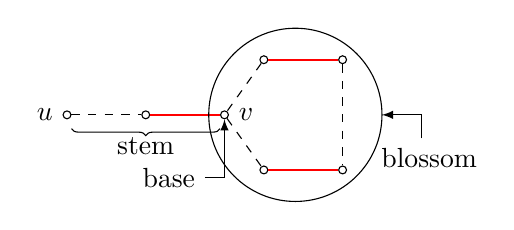
\begin{tikzpicture}[
				vertex/.style={circle, draw, inner sep=0pt, minimum size=1mm},
			]
			\node[vertex, label=left:{$u$}] (u) at (0,0) {};
			\node[vertex] (a) at (1,0) {};
			\node[vertex, label=right:{$v$}] (v) at (2,0) {};
			\node[vertex] (c1) at (2.5,0.7) {};
			\node[vertex] (c2) at (3.5,0.7) {};
			\node[vertex] (c3) at (3.5,-0.7) {};
			\node[vertex] (c4) at (2.5,-0.7) {};
			\draw[dashed] (u) -- (a);
			\draw[thick, red] (a) -- (v);
			\draw[dashed] (c1) -- (v) -- (c4);
			\draw[thick, red] (c1) -- (c2);
			\draw[thick,red] (c4) -- (c3);
			\draw[dashed] (c2) -- (c3);
			\draw[decoration={brace,mirror,raise=5pt},decorate] (u) -- node[midway, yshift=-0.4cm] {stem} (v);
			\draw[-latex] (1.75,-0.8) node[left]{base} -- (2,-0.8) -- (v);
			\draw (2.9,0) circle (1.1cm);
			\draw[-latex] (4.5,-0.3) node[below,xshift=0.1cm]{blossom} -- (4.5,0) -- (4,0);
		\end{tikzpicture}
	\end{minipage}
\end{Definition}

\begin{observation}
	For a flower since the stem is an even augmenting path the base of the blossom is even as well ass all the other vertices of the blossom are even.
\end{observation}

Since blossoms are in the way of getting augmenting paths we want to remove the blossoms from the graph.
\subsection{Shrinking Blossoms}
In order to remove the blossoms from the graph we will shrink the blossoms into a single vertex every time we encounter a blossom while constructing the augmenting tree.
\begin{question}{}{}
	How to shrink a blossom into a single vertex?
\end{question}

Let $B$ be a blossom in $G$. Then the new graph is $G?B=(V',E')$ where $$V'=(V\setminus B)\cup \{v_b\},\qquad E'=\Big(E\setminus\{(u,v)\colon u\in B\text{ or }v\in B\}\Big)\cup \{(u,v_b)\colon u\notin B, v\in B, (u,v)\in E\}$$ So if $M$ is a matching in $G$ then we can also a get a matching $M/B$  in $G/B$ from $M$ after shrinking $B$ into  a single vertex where $M/B=M\setminus \{\text{Matching edges in $B$}\}$.
\begin{Theorem}{}{}
	Let $B$ be a blossom wrt $M$. $M$ is a maximum matching in $G$ if and only if $M/B$ is a maximum matching in $G/B$.
\end{Theorem}
